Este capítulo descreve a metodologia adotada para investigar a formação e impacto de câmaras de eco na rede de usuários da aplicação Colab. A pesquisa é estruturada de forma iterativa e incremental, permitindo que cada etapa informe e refine as subsequentes.

\section{Natureza da Pesquisa}

A pesquisa adota uma abordagem tanto descritiva quanto exploratória, conforme delineado por \cite{2008_Yin_BOOK} e \cite{2007_Babbie_BOOK}.

A pesquisa descritiva, como sugerido por \cite{2007_Babbie_BOOK}, é empregada quando o objetivo é descrever características de um fenômeno ou a relação entre variáveis. No contexto deste estudo, a abordagem descritiva é utilizada para categorizar e detalhar os usuários do Colab, fornecendo uma representação clara e sistemática dos mesmos. Esta metodologia é particularmente útil para estabelecer um panorama claro do comportamento dos usuários, suas interações e padrões de linguagem, formando assim a base para análises subsequentes.

Por outro lado, a pesquisa exploratória, conforme descrito por \cite{2008_Yin_BOOK}, é frequentemente empregada quando o pesquisador tem pouco ou nenhum conhecimento prévio sobre o fenômeno em estudo. Ela busca descobrir padrões, ideias ou hipóteses, em vez de testar uma hipótese predefinida. No caso desta pesquisa, a abordagem exploratória é crucial para identificar e compreender as câmaras de eco dentro da rede do Colab, um fenômeno ainda pouco explorado na literatura. Esta abordagem permite uma investigação flexível, adaptando-se à medida que novas descobertas emergem.

A combinação dessas duas abordagens é estratégica. Enquanto a pesquisa descritiva fornece uma base sólida e detalhada sobre os usuários e suas interações, a pesquisa exploratória permite a descoberta de novos insights e compreensões sobre as câmaras de eco. Esta combinação maximiza a profundidade e amplitude da análise, garantindo que tanto os aspectos bem definidos quanto os emergentes do fenômeno sejam adequadamente abordados.

A metodologia deste estudo segue uma abordagem sequencial e iterativa, dividida em distintas fases interligadas. Cada fase é projetada para conduzir experimentos específicos que contribuem para uma compreensão mais profunda e abrangente das dinâmicas presentes na rede Colab.

Em cada fase, são definidos objetivos claros e hipóteses a serem testadas. A fase inicial se concentra na coleta e análise descritiva de dados do Colab, visando caracterizar os usuários, eventos e interações. Os resultados dessa fase são fundamentais para estabelecer uma base sólida e compreensível sobre o comportamento dos usuários.

À medida que avançamos para as fases subsequentes, os resultados dos experimentos anteriores são utilizados como insumos essenciais. Por exemplo, os dados coletados na primeira fase, que detalham as interações dos usuários, servem como base para a identificação das comunidades da rede na segunda fase. Os insights obtidos na segunda fase, por sua vez, orientam a seleção de tipos de eventos específicos a serem analisados na terceira fase.

Essa abordagem sequencial e iterativa permite que cada fase da pesquisa se beneficie das descobertas e conclusões anteriores, enriquecendo a análise e possibilitando insights mais profundos. Além disso, essa estratégia promove a construção gradual de conhecimento, à medida que cada experimento agrega informações e levanta novas questões a serem exploradas.

Em resumo, a pesquisa adota uma estratégia de fases interdependentes, em que os resultados de cada experimento alimentam o próximo, ampliando nosso entendimento das dinâmicas da rede Colab e das câmaras de eco presentes nesse ambiente

\section{Universo e Amostra}

Para a realização deste estudo, foram empregados dados providenciados pela equipe de Pesquisa e Desenvolvimento do Colab, abrangendo um universo significativo de 57.801 usuários ativos. O período de análise estende-se de Março de 2013 a Maio de 2022, proporcionando uma visão longitudinal do comportamento dos usuários e da evolução da rede. As cidades de Caruaru, Rio de Janeiro e Recife foram incluídas na análise para fornecer uma compreensão amplificada da topologia da rede e dos padrões de interação em diferentes contextos urbanos e demográficos.

Especificamente, o estudo concentrou-se com maior intensidade nas cidades de Niterói, Mesquita e Santo André, pois essas localidades apresentaram o maior volume de interações dentro da plataforma. A escolha dessas cidades como foco principal permite um exame detalhado das dinâmicas de interação que podem ser cruciais para a compreensão de fenômenos sociais complexos mediados pela plataforma.

Dentro da amostra selecionada, foram registradas 329.694 eventos e 334.682 comentários, totalizando 801.792 interações que servem como uma base robusta para análises subsequentes. Estes dados refletem a rica troca de informações e o engajamento dos usuários com o aplicativo, constituindo um campo fértil para investigações sobre a formação de comunidades, disseminação de informações e construção de consenso dentro do ambiente digital.

\section{Coleta de Dados}

Os dados analisados foram gentilmente disponibilizados pelo Colab em formato CSV, permitindo a manipulação e análise direta. Incluídos neste conjunto de dados estão as listas de arestas, que ilustram as relações entre os usuários, e uma série de atributos relacionados às atividades dos usuários na plataforma, tais como interações, postagens, além de informações demográficas e geográficas relevantes para o estudo. Importante ressaltar que os dados foram devidamente anonimizados para garantir a privacidade dos usuários, removendo quaisquer identificadores pessoais. Discutimos esse processo em \autoref{sec:anonimizacao}. A estruturação dos dados e os procedimentos de pré-processamento aplicados estão descritos no \autoref{sec:modelo_de_dados}, garantindo a transparência e a reprodutibilidade das análises realizadas.


\section{Procedimentos de Análise}

\begin{itemize}
	\item \textbf{Análise de Redes Sociais:} Utilizando técnicas de ciência de dados e análise de grafos para identificar estruturas e características da rede Colab.
	\item \textbf{Classificação de Usuários:} Serão empregadas técnicas de processamento de linguagem natural e aprendizado de máquina supervisionado para classificar postagens e comportamentos dos usuários.
	\item \textbf{Detecção de Câmaras de Eco:} Adaptação das heurísticas propostas por \cite{2023_Atiqi_BOOK} ao contexto do Colab, combinadas com técnicas de análise de redes e teoria dos grafos.
	\item \textbf{Simulações:} A Modelagem Baseada em Agentes (ABM) e simulações de Monte Carlo serão usadas para avaliar o impacto de diferentes cenários e intervenções na formação de câmaras de eco.
\end{itemize}

\begin{figure}
	\centering
	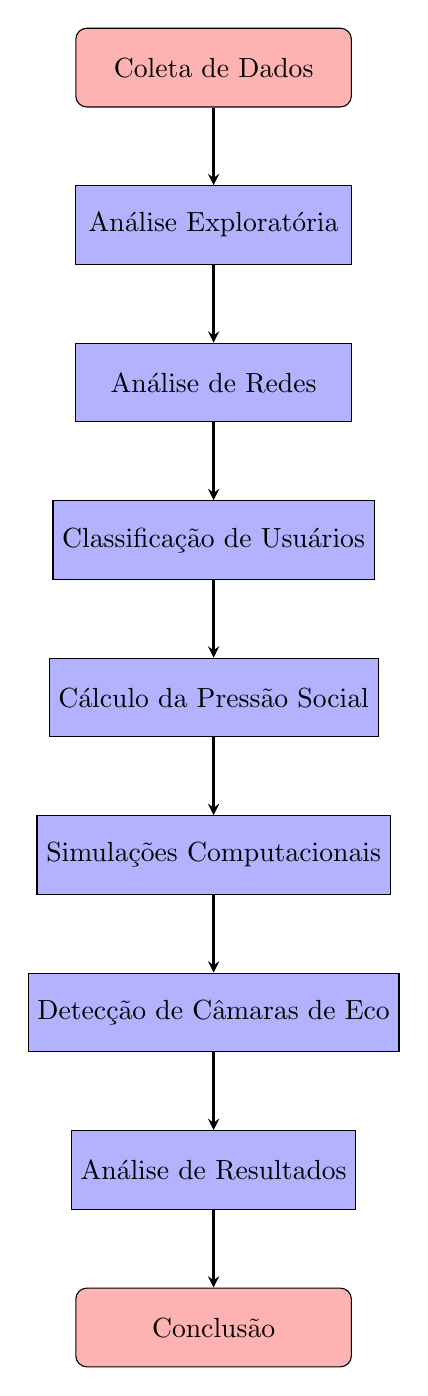
\begin{tikzpicture}[node distance=2cm]
		% Estilos para os nós
		\tikzstyle{startstop} = [rectangle, rounded corners, minimum width=3.5cm, minimum height=1cm, text centered, draw=black, fill=red!30]
		\tikzstyle{process} = [rectangle, minimum width=3.5cm, minimum height=1cm, text centered, draw=black, fill=blue!30]
		\tikzstyle{arrow} = [thick,->,>=stealth]
		% Nós
		\node (start) [startstop] {Coleta de Dados};
		\node (proc1) [process, below of=start] {Análise Exploratória};
		\node (proc2) [process, below of=proc1] {Análise de Redes};
		\node (proc3) [process, below of=proc2] {Classificação de Usuários};
		\node (proc4) [process, below of=proc3] {Cálculo da Pressão Social};
		\node (proc5) [process, below of=proc4] {Simulações Computacionais};
		\node (proc6) [process, below of=proc5] {Detecção de Câmaras de Eco};
		\node (proc7) [process, below of=proc6] {Análise de Resultados};
		\node (stop) [startstop, below of=proc7] {Conclusão};
		% Setas
		\draw [arrow] (start) -- (proc1);
		\draw [arrow] (proc1) -- (proc2);
		\draw [arrow] (proc2) -- (proc3);
		\draw [arrow] (proc3) -- (proc4);
		\draw [arrow] (proc4) -- (proc5);
		\draw [arrow] (proc5) -- (proc6);
		\draw [arrow] (proc6) -- (proc7);
		\draw [arrow] (proc7) -- (stop);
	\end{tikzpicture}
	\caption{Diagrama ilustrando os passos da metodologia.}
\end{figure}

\section{Ferramentas e Softwares}

\begin{itemize}
	\item Análise Exploratória de Redes com Gephi: Inicialmente, será conduzida uma análise exploratória de redes usando o software Gephi. Esta fase permitirá visualizar a estrutura da rede, identificar clusters e comunidades e também entender os padrões de interação entre os usuários.
	\item Análise de Redes com Python e NetworkX: Para um exame mais detalhado e uma análise quantitativa da rede, utilizaremos Python, especificamente a biblioteca NetworkX. Com isso, esperamos identificar métricas-chave da rede, como centralidade, densidade e modularidade. Esse estudo nos ajudará a identificar as câmaras de eco e seus nós principais.
	\item Técnicas de Simulação: A modelagem baseada em agentes e a simulação com modelos ERGM serão empregadas para simular o comportamento dos usuários e a propagação de informações. Isso nos permitirá prever a propagação de informações dentro e entre câmaras de eco e tentar entender as dinâmicas que levam à formação desses grupos.
	\item Ambiente de Desenvolvimento Google Colaboratory: Todas as análises computacionais e o desenvolvimento de algoritmos serão realizados no ambiente Google Colaboratory, que oferece um ambiente de codificação interativo e colaborativo baseado na nuvem. Isso facilitará a reproducibilidade da pesquisa e também a colaboração com outros pesquisadores.
\end{itemize}

\section{Aspectos Éticos e Anonimização}
\label{sec:anonimizacao}

A pesquisa assegura a anonimidade e a privacidade das informações pessoais dos usuários. Reconhecendo a importância crítica da proteção de dados, aplicamos uma abordagem de anonimização rigorosa e meticulosa. A conformidade com regulamentações de proteção de dados, como a \sigla{$LGPD$}{Lei Geral de Proteção de Dados do Brasil, é a legislação que regula a coleta, armazenamento e tratamento de dados pessoais, visando proteger a privacidade e os direitos dos indivíduos.}, é priorizada para garantir que todos os dados coletados e analisados sejam tratados de acordo com as normas éticas e legais.

Utilizamos técnicas avançadas de Processamento de Linguagem Natural (\sigla{$PLN$}{Processamento de Linguagem Natural, é uma área da inteligência artificial que foca na interação entre computadores e a linguagem humana, visando à compreensão e geração de linguagem natural por máquinas.}), especificamente com a biblioteca spaCy, para identificar e remover informações pessoais dos dados textuais. Um sistema de anonimização, \texttt{MessageSanitizer}, foi desenvolvido para este propósito. Este sistema utiliza um modelo de PLN treinado em português para reconhecer e substituir nomes de pessoas, organizações, e-mails e números de telefone por marcadores não identificáveis. Além disso, padrões regulares são aplicados para capturar e anonimizar qualquer dado sensível que possa ter escapado à detecção do modelo de PLN. Além de remover entidades identificáveis, \texttt{MessageSanitizer} realiza uma limpeza adicional de dados, removendo stopwords, pontuações e números, e aplicando lematização para reduzir as palavras às suas formas base, facilitando análises subsequentes e evitando a identificação indireta de usuários. Stopwords customizadas foram adicionadas para excluir referências específicas a locais que poderiam levar à identificação de indivíduos ou grupos.

A integridade dos dados é mantida, assegurando que as informações anonimizadas permaneçam significativas e úteis para a análise sem comprometer a identidade dos usuários. Este processo é transparente e repetível, garantindo que outros pesquisadores possam validar e reproduzir os métodos de anonimização aplicados.

\section{Limitações}

Embora esta pesquisa forneça insights valiosos sobre a dinâmica de formação de câmaras de eco no Colab, sua aplicabilidade é intrinsecamente ligada às particularidades desta plataforma. O Colab, com sua base de usuários específica e contexto de e-Government brasileiro, pode comportar-se de maneira distinta em comparação a outras redes sociais com diferentes propósitos ou contextos culturais e políticos. Além disso, a concentração no idioma português pode restringir a generalização dos resultados para comunidades linguísticas distintas, em que nuances culturais e semânticas influenciam o comportamento online e a formação de discursos polarizados.

No entanto, a metodologia empregada é projetada para ser adaptável a outros contextos, desde que sejam fornecidos dados equivalentes. As listas de arestas e nós, fundamentais para reconstruir a estrutura da rede social, podem ser geradas em qualquer plataforma que permita a exportação de interações e informações de perfil dos usuários em formatos padronizados como CSV. A análise de conteúdo, enquanto centrada em postagens em português, pode ser replicada em outras línguas com as ferramentas de processamento de linguagem natural apropriadas, contanto que sejam consideradas as variações linguísticas e culturais relevantes.

Ademais, é imperativo considerar as implicações éticas ao expandir esta pesquisa para novos contextos, assegurando a proteção da privacidade dos usuários e o cumprimento das diretrizes de pesquisa responsável. Dessa forma, a reprodutibilidade desta pesquisa em outras plataformas e idiomas é viável, com a compreensão de que adaptações metodológicas podem ser necessárias para acomodar diferenças estruturais e culturais.
